\documentclass[final]{beamer}

% ====================
% Packages
% ====================

\usepackage[T1]{fontenc}
\usepackage{lmodern}
\usepackage[size=a0,scale=1.0]{beamerposter}
\usetheme{gemini}
\usecolortheme{ITNU}
\usepackage{graphicx}
\usepackage{booktabs}
\usepackage{svg}
\usepackage{pgfplots}

% for circling parts
\usepackage{graphicx}
\usepackage[usestackEOL]{stackengine}
\usepackage{xcolor}
\def\calloutsym{%
  \ensurestackMath{%
  \scalebox{3.5}{\color{red}\stackunder[0pt]{\bigcirc}{\downarrow}}}%
}
\newcommand\callouttext[1]{%
  \def\stacktype{S}\renewcommand\useanchorwidth{T}\stackText%
  \stackunder{\calloutsym}{\scriptsize\Longstack{#1}}\stackMath%
}
\newcommand\callout[3][1.5pt]{%
  \def\stacktype{L}\stackMath\stackunder[#1]{#2}{\callouttext{#3}}%
}

% ====================
% Lengths
% ====================

% If you have N columns, choose \sepwidth and \colwidth such that
% (N+1)*\sepwidth + N*\colwidth = \paperwidth
\newlength{\sepwidth}
\newlength{\colwidth}
\setlength{\sepwidth}{0.001\paperwidth}
\setlength{\colwidth}{0.3\paperwidth}

\newcommand{\separatorcolumn}{\begin{column}{\sepwidth}\end{column}}

% ====================
% Title
% ====================

\title{CS6216 Project Report: Stein Variational Gradient Descent}

\author{Apivich Hemachandra\inst{1} \and
Jiashu Tao\inst{1} \and
Bo Wang\inst{1}   \and
Jiayuan Ye\inst{1} }
\institute{Department of Computer Science,  National University of Singapore\\{\small\textsuperscript{*}Alphabetical Order.}}

% remove this section if poster is for inhouse project
\addtobeamertemplate{headline}{} 
{
    \begin{tikzpicture}[remember picture,overlay]
    % tweak these sizes according to the logo of the company:
    % xshift, yshift, height
    \node [anchor=north west, inner sep=3cm] at ([xshift=-1.5cm,yshift=-0.8cm]current page.north west)     {
\includegraphics[height=3cm]{imgs/logo.png}}; 
    \end{tikzpicture} 
}

% ====================
% Body
% ====================

\begin{document}

\begin{frame}[t]
\begin{columns}[t]

\separatorcolumn

\begin{column}{\colwidth}

\begin{block}{Problem Setting}

\end{block}

\begin{block}{SVGD Algorithm}

SVGD \cite{liu2016stein}
\end{block}

  \begin{block}{Experiment: Toy Example}
  \textbf{Toy Example:} 1d gaussian mixture
    \begin{itemize}
     \item xxx
    \end{itemize}
    
\newcommand{\toyfigwidth}{0.9\textwidth}
\begin{figure}[!htbp]
    \centering
    % \begin{tabular}{@{}c@{}}
    %     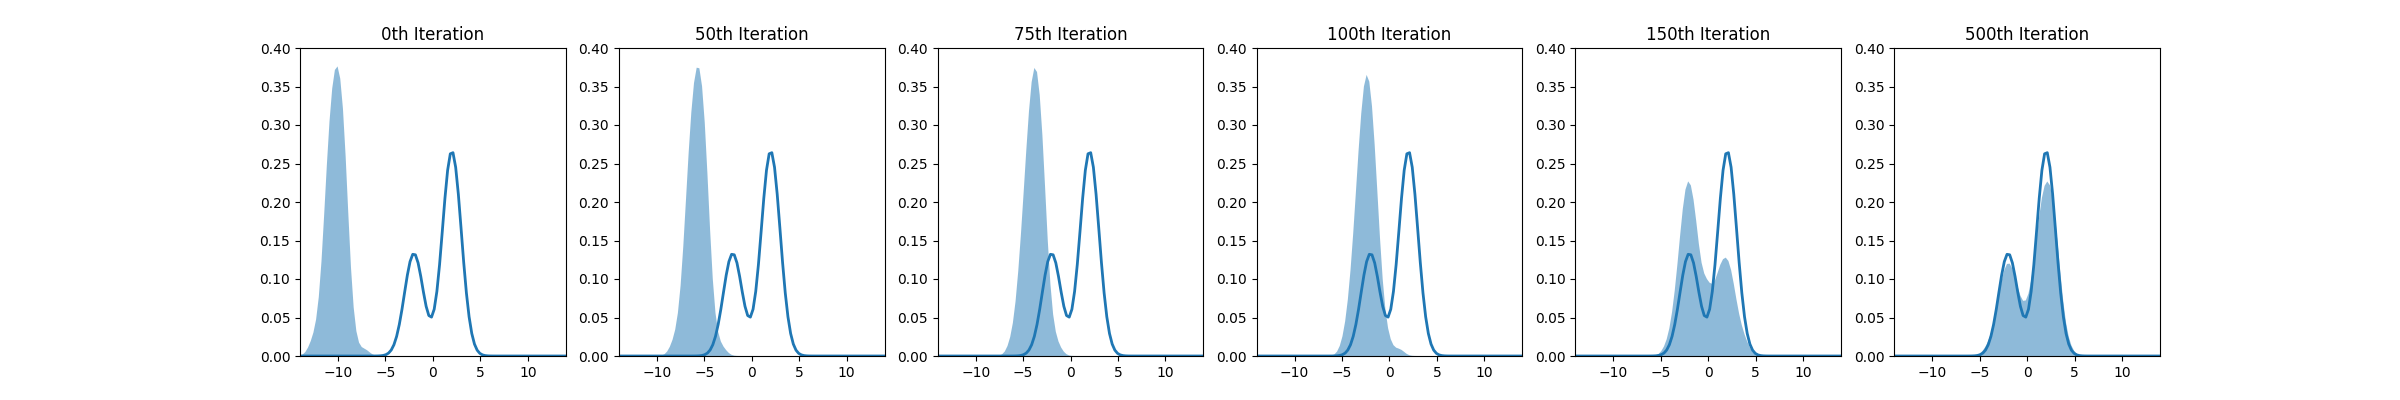
\includegraphics[width=\toyfigwidth]{figs/toy-figure1_step0.1_mu2.0_w0.33_gaussian.png} \\
    %     \small (1) StepSize = 0.1, 500 iterations, $\mu = \pm 2$, $(w_1, w_2) = (0.33, 0.67)$
    % \end{tabular}
    
    \begin{tabular}{@{}c@{}}
        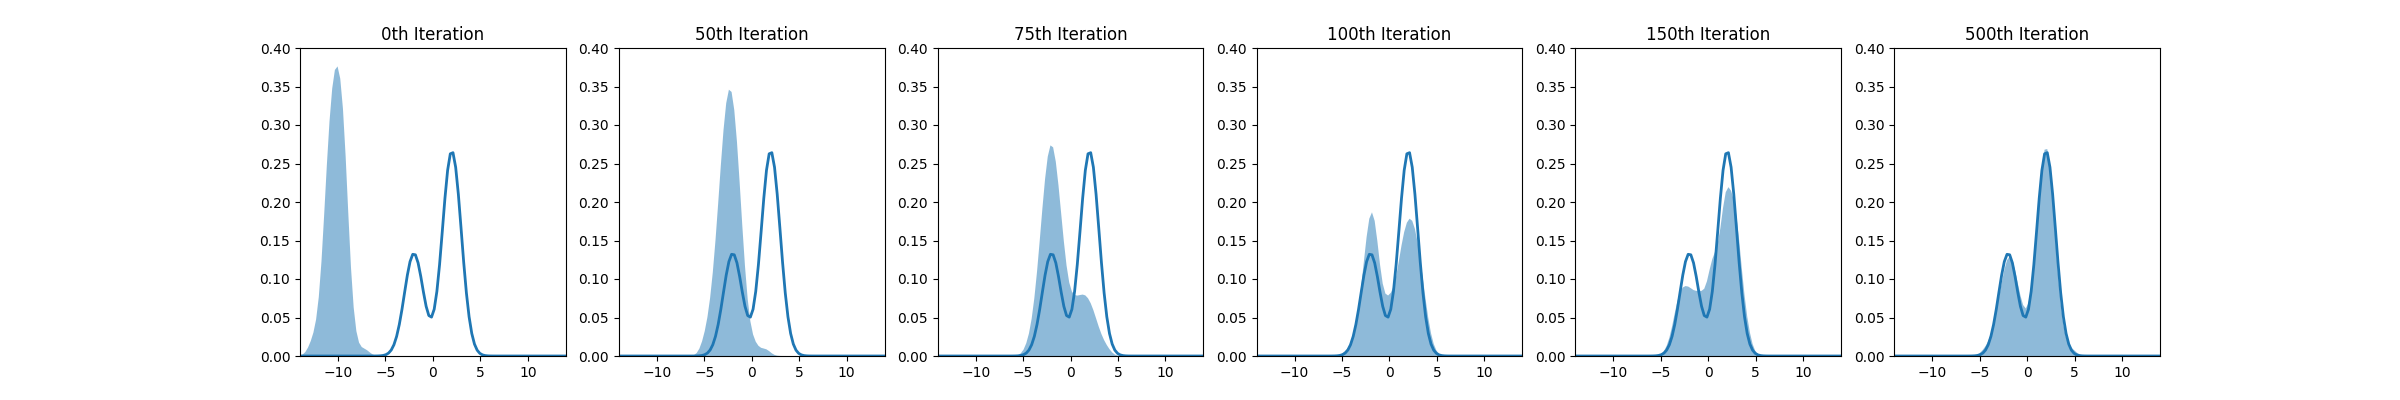
\includegraphics[width=\toyfigwidth]{figs/toy-figure1.png} \\
        \small (1) StepSize = 0.25, 500 iterations, $\mu = \pm 2$, $(w_1, w_2) = (0.33, 0.67)$
    \end{tabular}
    %\vspace{\floatsep}
    
    \begin{tabular}{@{}c@{}}
        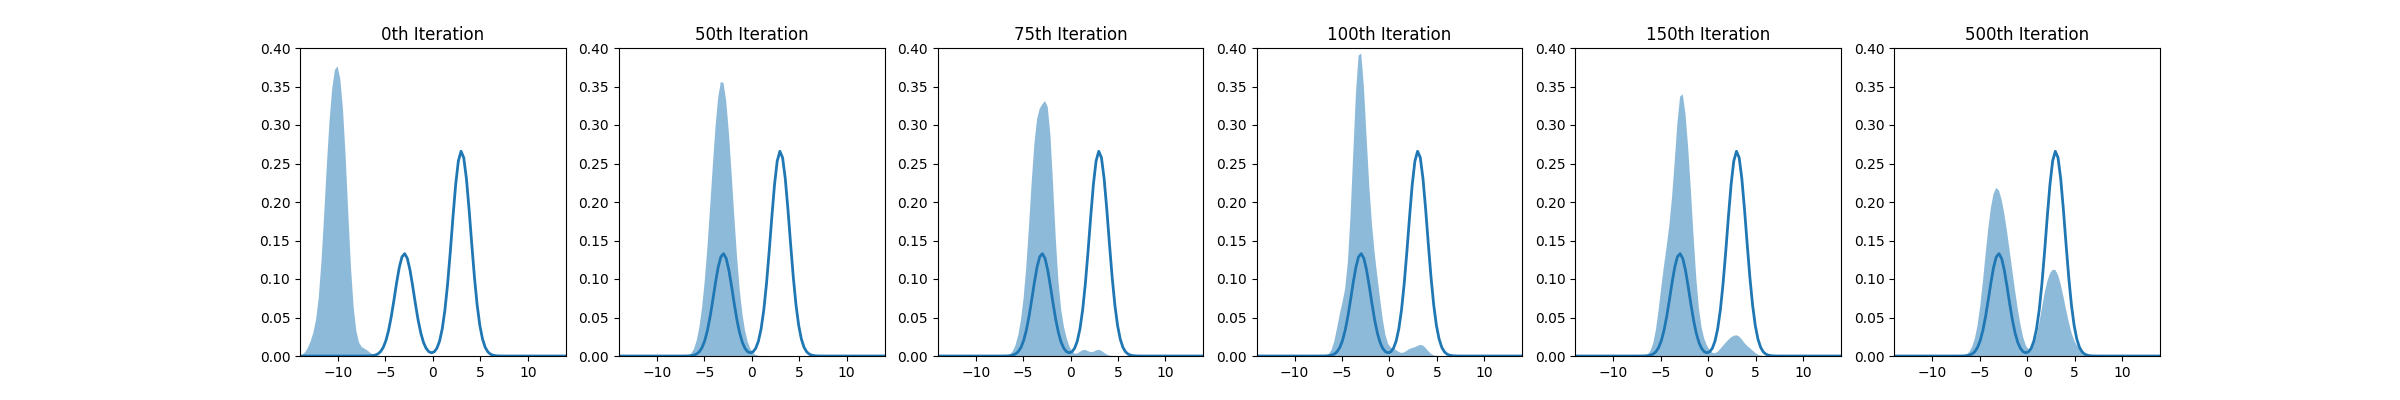
\includegraphics[width=\toyfigwidth]{figs/toy-figure1_step0.25_mu3.0_w0.33_gaussian.png} \\
        \small (2) StepSize = 0.25, 500 iterations, $\mu = \pm 3$, $(w_1, w_2) = (0.33, 0.67)$
    \end{tabular}
    
    \begin{tabular}{@{}c@{}}
        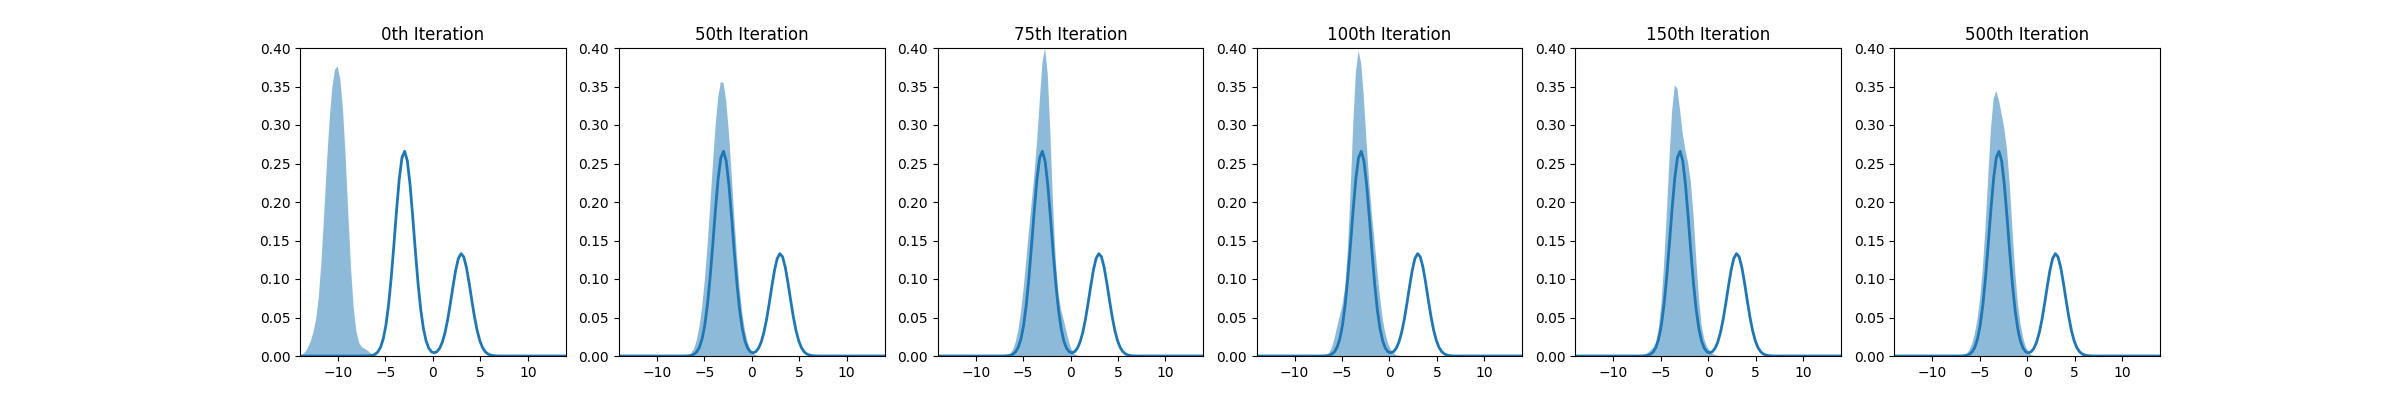
\includegraphics[width=\toyfigwidth]{figs/toy-figure1_step0.25_mu3.0_w0.67_gaussian.png} \\
        \small (3) StepSize = 0.25, 500 iterations, $\mu = \pm 3$, $(w_1, w_2) = (0.67, 0.33)$
    \end{tabular}
    
    % \begin{tabular}{@{}c@{}}
    %     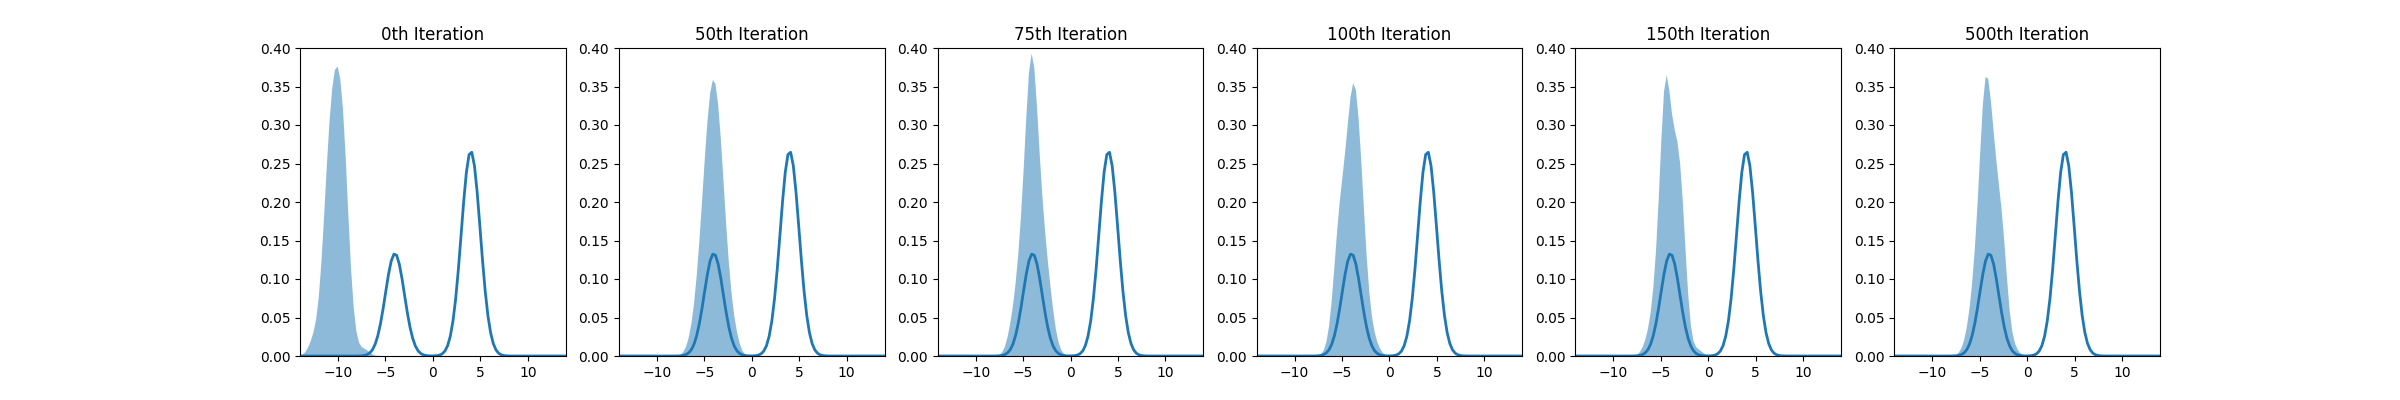
\includegraphics[width=\textwidth]{figs/toy-figure1_step0.25_mu4.0_w0.33_gaussian.png} \\
    %     \small (5) StepSize = 0.25, $\mu = \pm 4$, $(w_1, w_2) = (0.33, 0.67)$
    % \end{tabular}
    
    \begin{tabular}{@{}c@{}}
        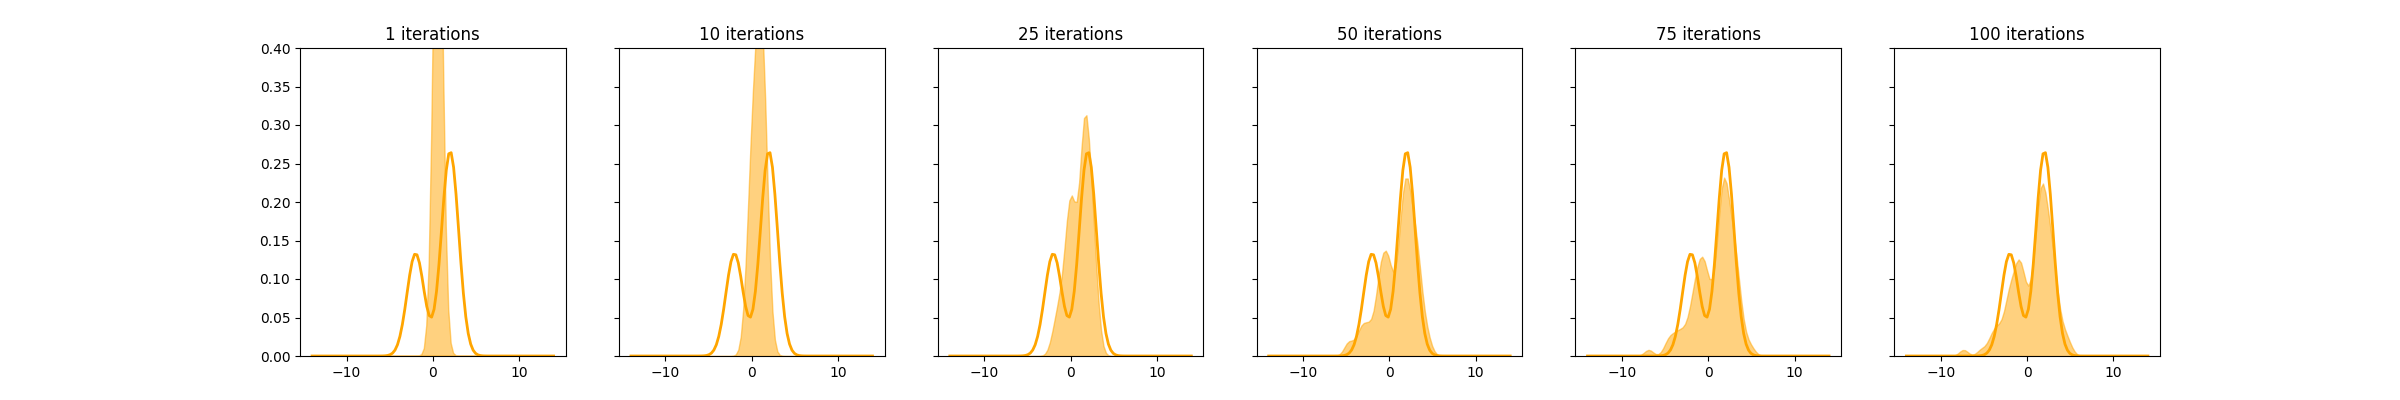
\includegraphics[width=\toyfigwidth]{figs/toy-figure1-numpyro.png} \\
        \small (4) ELBO Loss (NumPyro) StepSize = 0.1, 100 iters, $\mu = \pm 3$, $(w_1, w_2) = (0.33, 0.67)$
    \end{tabular}
     
    \caption{Toy example with 1D Gaussian mixture. Particle densities are visualized by KDE.}
    \label{fig:toy1dgaussian}
\end{figure}

    \begin{figure}[!htbp]
    \centering
    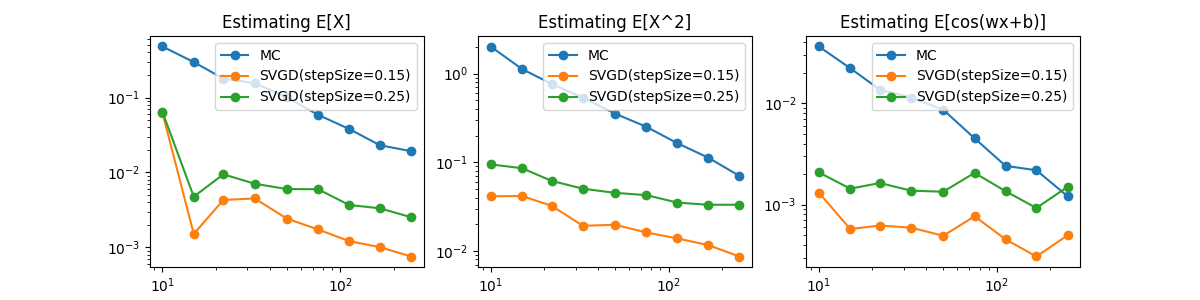
\includegraphics[width=\textwidth]{figs/toy-figure2-merged.png}
    \caption{Comparison between MC and SVGD on simple mean estimation tasks. }
    \label{fig:my_label}
\end{figure}

  \end{block}
  


\end{column}

\separatorcolumn

\begin{column}{\colwidth}

  \begin{block}{Experiment: Execution Time vs \#Particles}
  \textbf{Toy Example:} Estimating mean of multivariate Gaussian
    \begin{itemize}
     \item xxx
    \end{itemize}
     \begin{figure}[!htbp]
    \centering
    \begin{tabular}{@{}cc@{}}
            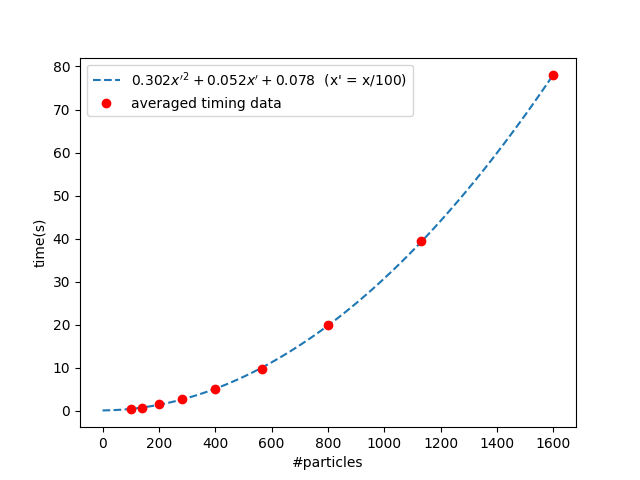
\includegraphics[width=0.40\textwidth]{figs/toy-timing-particles.png} & 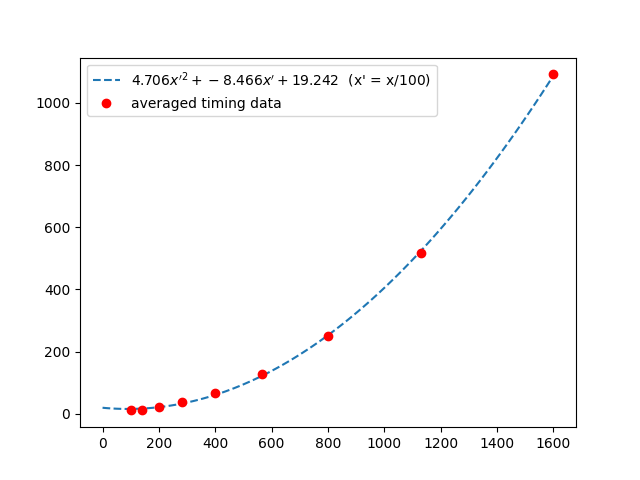
\includegraphics[width=0.40\textwidth]{figs/toy-timing-particles-numpyro-elbo.png}\\
        \small Original SVGD & NumPyro (ELBO Loss) \\
    \end{tabular}
    \caption{Timing vs particles }
    \label{fig:timingparticles}
\end{figure}

  \end{block}

\begin{block}{Experiment: Linear Regression}
  \textbf{Linear Regression:} Linear Regression
    \begin{itemize}
     \item xxx
    \end{itemize}
     \begin{figure}[h]
    \centering
    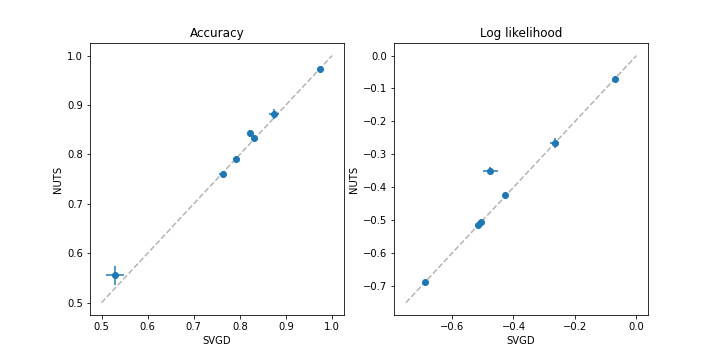
\includegraphics[width=0.6\textwidth]{figs/logistic_svgd_nuts.png}
    \caption{Comparison of accuracy (left) and log-likelihood (right) obtained by NUTS and SVGD algorithm on small-scale logistic regression dataset. The dotted line represents the situation where both algorithms perform as well was each other, and each point represent the average result on one of the dataset.}
    \label{fig:logist_small}
\end{figure}
  \end{block}

\end{column}

\separatorcolumn

\begin{column}{\colwidth}

\begin{block}{Summary}
\end{block}

  \begin{block}{References}

    \nocite{*}
    \footnotesize{\bibliographystyle{plain}\bibliography{poster}}

  \end{block}
  
\end{column}

\separatorcolumn

\end{columns}
\end{frame}

\end{document}